\chapter{Arduino}\label{analysis:arduino}
Arduino was created by the Interaction Design Institute Ivrea (Italy), by Massimo Banzi and David Cuartielles. They were looking for an easy and cheap way for students, who study design, to integrate micro controllers into their projects\cite{arduino:hist}. Both the board and the programming language was based on the works of Hernando Barragán, one of Massimo Banzi master thesis students \cite{Wiring:thesis}.

In this project Arduino board is used to execute the code, and show a type of output. The output will be in the form of a LCD Display. 

\section{The Hardware Components}
Arduino is a single-board micro-controller, see figure \ref{fig:Arduino_uno}.
A board consists of open source hardware, which is designed around an 8-bit Atmel AVR micro-controller. Arduino boards varies in sizes. Arduino Uno board for example, has a max width of 2.1'' (5,33cm) and a length of 2.7'' (6,86cm).  \\

\par
\raisebox{-.5\height}{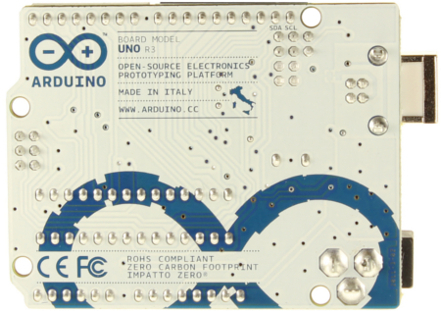
\includegraphics[width=6.5cm]{billeder/ArduinoUno_R3_Back_450px.jpg}}
\hfill
\raisebox{-.5\height}{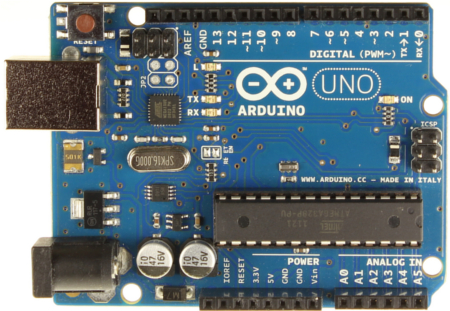
\includegraphics[width=6.5cm]{billeder/ArduinoUno_R3_Front_450px.jpg}}
\begin{figure}[H]
\caption{Picture of back- and fronside of the Arduino Uno board \cite{Arduino:board_pics}}
\label{fig:Arduino_uno}
\end{figure}
\par

\par
\raisebox{-.5\height}{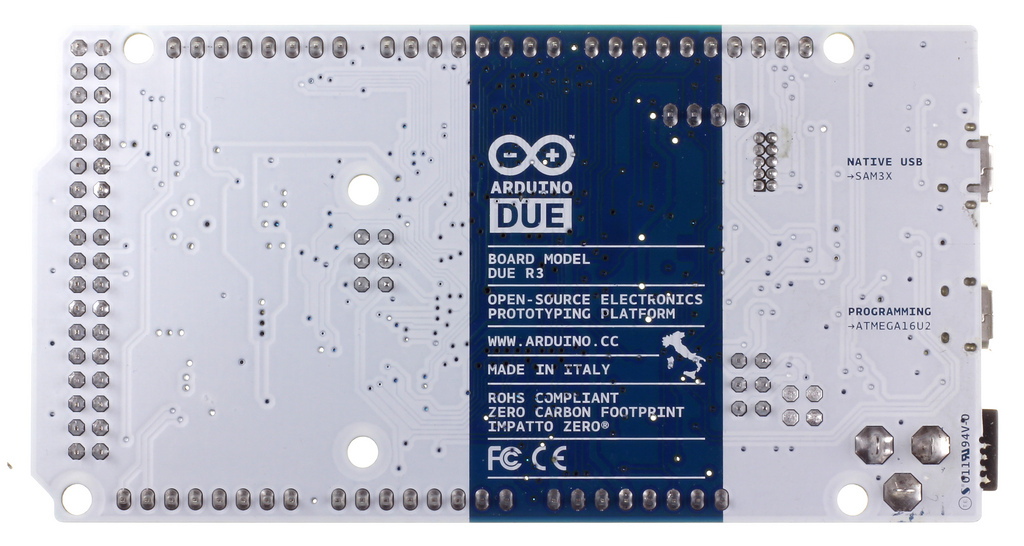
\includegraphics[width=6.5cm]{billeder/ArduinoDue_2.jpg}}
\hfill
\raisebox{-.5\height}{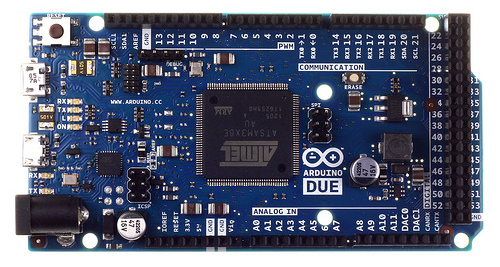
\includegraphics[width=6.5cm]{billeder/ArduinoDue_1.jpg}}
\begin{figure}[H]
\caption{Picture of back- and fronside of the Arduino Duo board \cite{Arduino:board_pics}}
\label{fig:Arduino_duo}
\end{figure}
\par

\subsection*{Specifications}
The board provides some input and output possibilities. The Arduino Uno, figure \ref{fig:Arduino_uno}, has 14 digital I/O and 6 analog inputs, where as the Arduino Due, figure \ref{fig:Arduino_duo}, has 54 digital, and 12 analog pins. The I/O functions are placed on top of the board, and are freely accessible, and consist of 0.1'' female headers. Besides the I/O there is also a Power connector, which almost in all cases require 5 volt DC. There is an USB connection on the board, so that processing data to the micro-controller is possible, though it is shown as a virtual com-port on the connected computer. However, on older boards, instead of the USB connection, a RS232 were used for serial communication. 

\begin{figure}[H]
\centering
\begin{tabular}{|c|c|}
\hline 
Microcontroller & ATmega328 \\ 
\hline 
Operating Voltage & 5V \\ 
\hline 
Input Voltage (recommended)	 & 7-12V \\ 
\hline 
Input Voltage (limits) & 6-20V \\ 
\hline 
Digital I/O Pins & 14 (of which 6 provide PWM output) \\ 
\hline 
Analog Input Pins & 6 \\ 
\hline 
DC Current per I/O Pin & 40 mA \\ 
\hline 
DC Current for 3.3V Pin & 50 mA \\ 
\hline 
Flash Memory & 32 KB (ATmega328) of which 0.5 KB used by bootloader \\ 
\hline 
SRAM & 2 KB (ATmega328) \\ 
\hline 
EEPROM & 1 KB (ATmega328) \\ 
\hline 
Clock Speed & 16 MHz \\ 
\hline 
\end{tabular} 
\caption{Hardware specifications for the Arduino Uno}
\end{figure}

On the board there is a LED, which is connected to the digital pin 13. When this diode is set to ``HIGH'' it will be turned on, and if its value is ``LOW'' it turns off. Besides the LED, there is also a reset button. If the button is pressed the micro-controller is reset. 

The specifications, which are important to take into consideration in regard to designing a programming language aimed at the Arduino platform, is the flash memory, the main memory(SRAM) and the CPU speed. The most limiting factor to take into consideration is the amount of RAM, the larger and more complex the data structures are, the bigger the risk of running out of memory while executing a program. Although this is not limited to developing for the Arduino platform, it is certainly a larger factor, then when developing for desktop computers.
Another factor that need attention is the flash memory, meaning the pace available for the program, the smallest example code for the Arduino, the Blink example listings \ref{lst:blink}, only uses 1084 bytes, which is approximately $3.3 \%$ of the total memory available. 

\begin{table}[h!]\scriptsize
\centering
\begin{tabular}{cc} 
\begin{minipage}{6cm}
{\begin{lstlisting}[caption=Arduino,frame=none,resetmargins=true,label={lst:blink}]
int led = 13;
void setup() {                
  pinMode(led, OUTPUT);     
}

void loop() {
  digitalWrite(led, HIGH);   
  delay(1000);    
  digitalWrite(led, LOW);  
  delay(1000);
}
\end{lstlisting}}
\end{minipage}
  & 
\begin{minipage}{10cm}
{\begin{lstlisting}[caption=C\#,frame=none,resetmargins=true,label={lst:C_hello}]
namespace hello
{
  class Program
  {
    static void Main(string[] args)
    {
       System.Console.WriteLine("Hello, World!");
       System.Console.ReadKey();
    }
  }
}
\end{lstlisting}}
  \end{minipage}
 \\ 
 \end{tabular} 
 \caption{Comparison between a simple Arduino and C\# example}
 \end{table} 

If a language has a lot of complex features, it will quickly run out of space. For instance with more complex languages like C\#, a simple hello world, listings \ref{lst:C_hello}, program uses 5120 bytes, and they can quickly run in the hundreds or thousands of kilobytes. This is even more important to remember, when one takes into account, that there are many different Arduino configurations, and the language have to function on all of them. The Arduino Nano for instance, only has 16 KB of memory, and there are Arduino clones by other manufactures with even less.



\subsection*{Components}
What makes Arduino such a good platform for beginners to learn to program on, is because it is really easy to connect a wide variety of components to it, making it possible for the Arduino to interact with the real world.

\begin{itemize}
\item[] \textbf{LED's} come in all size, shapes and colors, ranging from small pin size single color LED's, to large multi color LED displays.
\begin{figure}[H]
\centering
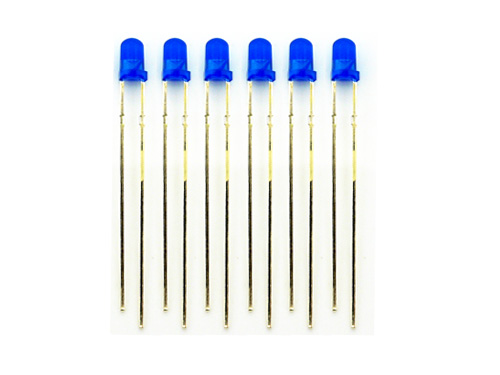
\includegraphics[width=5cm]{billeder/led.jpg}
\caption{3mm blue led}
\end{figure}
\item[] \textbf{Sensors} are some of the main components behind the Arduino success. They give the Arduino the ability to sense its surroundings. For instance the temperature of the room, whether the light is on of off, even advanced sensors like humidity, or gas sensor.
\begin{figure}[H]
\centering
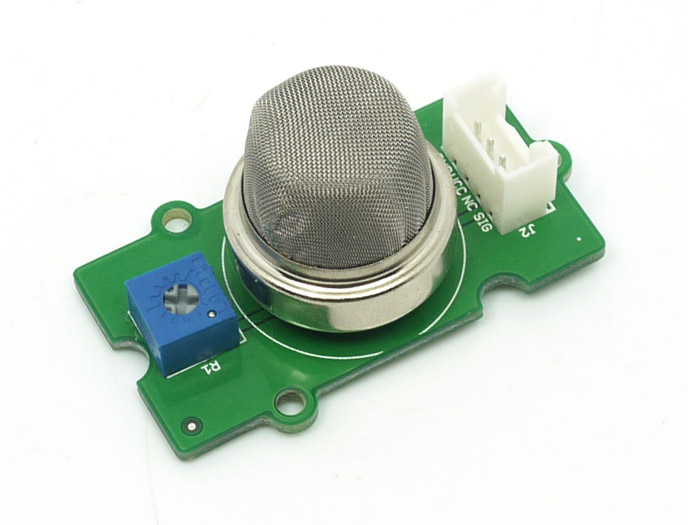
\includegraphics[width=5cm]{billeder/Sensor.jpg}
\caption{Gas sensor}
\end{figure}
\item[] \textbf{Motors} gives Arduino the ability to manipulate its surrounding, and act on the informations obtained from the sensors. There are two kind of motors, normal motors which can just be turned on/off. They are great for powering wheels or tracks. There are stepper motors, with these it is possible to control the exact amount of rotation. A more advanced version of the stepper motors are servo motors, with which more precise control is possible.
\begin{figure}[H]
\centering
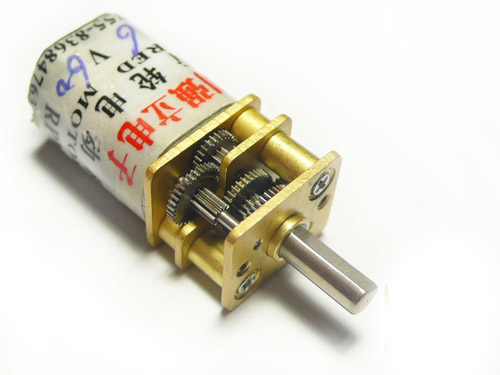
\includegraphics[width=5cm]{billeder/Motor.jpg}
\caption{Geared stepper motor}
\end{figure}
\item[] \textbf{Displays} are available in a wide range. Ranging from simple 2 line mono color LCD displays, all the way up to large OLED color and touch displays. 
\begin{figure}[H]
\centering
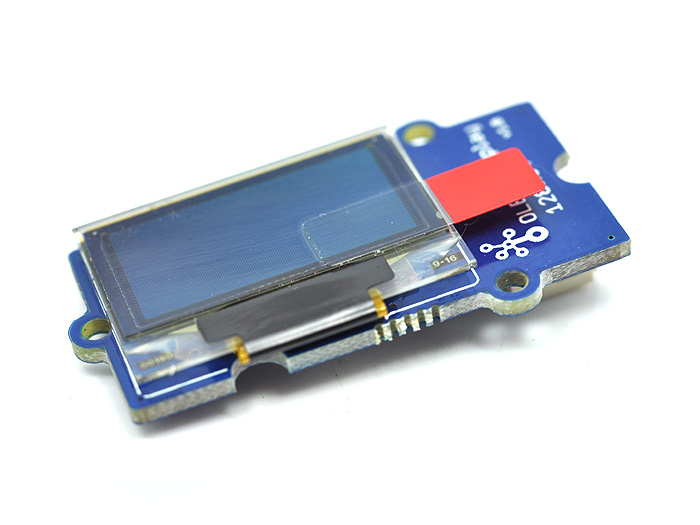
\includegraphics[width=5cm]{billeder/display.jpg}
\caption{OLED touch display}
\end{figure}
\item[] \textbf{Communication} components are easy to connect up on Arduino. This is allows it to communicate with other devices through either RF signals, Bluetooth, WiFi, cellular or just Ethernet connection.
\begin{figure}[H]
\centering
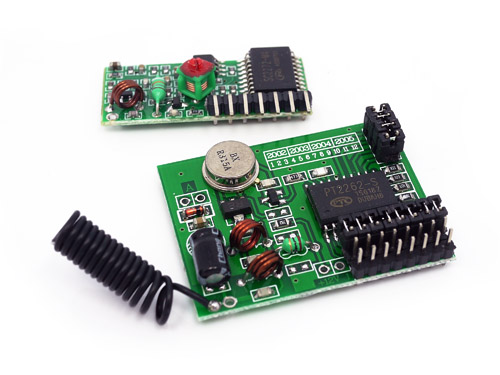
\includegraphics[width=5cm]{billeder/com.jpg}
\caption{RF transmitter and reciever}
\end{figure}
\item[] \textbf{Shields} are the components that makes the Arduino Platform great. They offer great  to the platform by allowing them to be plugged directly on to the Arduino. This makes it possible for anyone without any experience in electronics  to use them Shields are boards much like Arduino itself, but they offer all the capabilities of the components mentioned above.
\begin{figure}[H]
\centering
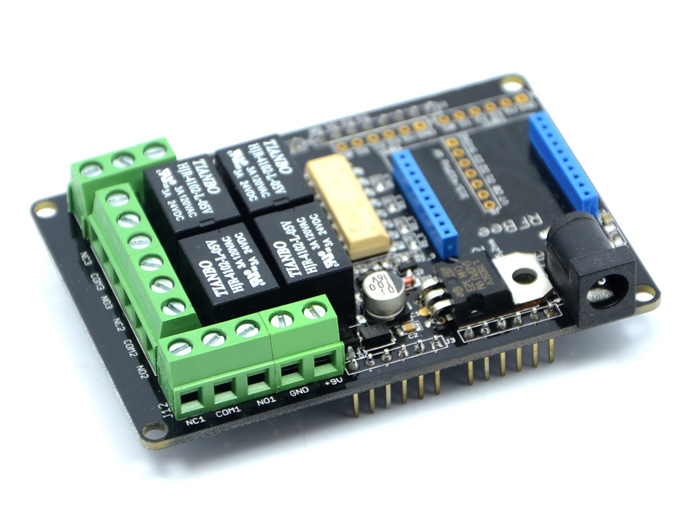
\includegraphics[width=5cm]{billeder/Shield.jpg}
\caption{Relay shield}
\end{figure}

\end{itemize}


